%
% markov.tex -- diskrete Markov-Ketten und Übergangsmatrizen
%
% (c) 2020 Prof Dr Andreas Müller, Hochschule Rapperswil
%
\section{Diskrete Markov-Ketten und Wahrscheinlichkeitsmatrizen
\label{buch:section:diskrete-markov-ketten}}
\rhead{Diskrete Markov-Ketten}
Die einführend im Abschnitt~\ref{buch:section:google-matrix}
vorgestellte Google-Matrix ist nur ein Beispiel für ein
Modell eines stochastischen Prozesses, der mit Hilfe von Matrizen
modelliert werden kann.
In diesem Abschnitt soll diese Art von Prozessen etwas formalisiert
werden.

%
% Beschreibung der Markov-Eigenschaft
% 
\subsection{Markov-Eigenschaft}
Ein stochastischer Prozess ist eine Familie von Zufallsvariablen
\index{stochastischer Prozess}%
\index{Prozess, stochastisch}%
\index{Zufallsvariable}%
$X_t$ mit Werten in einer Menge $\mathcal{S}$ von Zuständen.
Der Parameter $t$ wird üblicherweise als die Zeit interpretiert,
er kann beliebige reelle oder diskrete Werte annehmen, im letzten
Fall spricht man von einem Prozess mit diskreter Zeit.

Das Ereignis $\{X_t=x\}$ wird gelesen als ``zur Zeit $t$ befindet sich
der Prozess im Zustand $x$''.
Mit $P(X_t = x)$ wir die Wahrscheinlichkeit bezeichnet, dass sich
der Prozess zur Zeit $t$ im Zustand $x$ befindet.
Die Funktion $t\mapsto X_t$ beschreibt also den zeitlichen Ablauf
der vom Prozess durchlaufenen Zustände.
Dies ermöglicht, Fragen nach dem Einfluss früherer Zustände,
also des Eintretens eines Ereignisses $\{X_{t_0}=x\}$, auf das Eintreten eines
Zustands $s\in\mathcal{S}$ zu einem späteren Zeitpunkt $t_1>t_0$
zu studieren.
Das Ereignis $\{X_t = x\}$ kann man sich als abhängig von der Vorgeschichte
vorstellen.
\index{Vorgeschichte}%
Die Vorgeschichte besteht dabei aus dem Eintreten gewisser Ereignisse
\[
\{X_0=x_0\},\;
\{X_1=x_1\},\;
\{X_2=x_2\},\;
\dots,\;
\{X_n=x_n\}
\]
zu früheren Zeiten $t_0<t_1<\dots<t_n<t$.
Die bedingte Wahrscheinlichkeit
\begin{equation}
P(X_t = x \mid
X_{t_n}=x_n\wedge X_{t_{n-1}}=x_{n-1}\wedge\ldots\wedge X_{t_1}=x_1\wedge
X_{t_0}=x_0)
\label{buch:wahrscheinlichkeit:eqn:historybedingt}
\end{equation}
ist die Wahrscheinlichkeit dafür, dass der Prozess zur Zeit $t$ den
Zustand $x$ erreicht, wenn er zu den Zeitpunkten $t_0,t_1,\dots,t_n$
die Zustände $x_0,x_1,\dots,x_n$ durchlaufen hat.

\subsubsection{Gedächtnislosigkeit}
\index{Markov-Eigenschaft}%
In vielen Fällen ist nur der letzte durchlaufene Zustand wichtig.
Die Zustände zu den Zeitpunkten $t_0<\dots<t_{n-1}$ haben dann keinen
Einfluss auf die Wahrscheinlichkeit.
Auf die bedingte
Wahrscheinlichkeit~\eqref{buch:wahrscheinlichkeit:eqn:historybedingt}
sollten also die Ereignisse $\{X_{t_0}=x_0\}$ bis $\{X_{t_{n-1}}=x_{n-1}\}$
keinen Einfluss haben.

\begin{definition}
Ein stochastischer Prozess erfüllt die {\em Markov-Eigenschaft}, wenn 
für jede Folge von früheren Zeitpunkten $t_0<t_1<\dots <t_n<t$ und Zuständen
$x_0,\dots,x_n,x\in \mathcal{S}$ die 
Wahrscheinlichkeit~\eqref{buch:wahrscheinlichkeit:eqn:historybedingt}
nicht von der Vorgeschichte abhängt, also
\[
P(X_t = x\mid
X_{t_n}=x_n\wedge X_{t_{n-1}}=x_{n-1}\wedge\dots\wedge X_{t_1}=x_1\wedge
X_{t_0}=x_0)
=
P(X_t = x \mid
X_{t_n}=x_n).
\]
\index{Markov-Eigenschaft}
\end{definition}

Die Wahrscheinlichkeiten $P(X_t=x\mid X_s=y)$ mit $t>s$ bestimmen das
zeitliche Verhalten der Wahrscheinlichkeiten vollständig.
Wir schreiben daher auch
\[
p_{xy}(t, s)
=
P(X_t = x\mid X_s=y)
\]
für die sogenannte {\em transiente Übergangswahrscheinlichkeit}.
\index{transiente Übergangswahrscheinlichkeit}%
Für eine endliche Menge von Zuständen, können die transienten
Übergangswahrscheinlichkeiten auch als zeitabhängige 
quadratische Matrix $P(s,t)$ geschrieben werden, deren
Einträge
\[
(P(s,t))_{xy}
=
p_{xy}(t,s)
\]
mit den Zuständen $x,y\in\mathcal{S}$ indiziert sind.

\subsubsection{Die Chapman-Kolmogorov-Gleichung}
\index{Chapman-Kolmogorov-Gleichung}%
Man beachte, dass in der Definition der Markov-Eigenschaft
keine Voraussetzungen darüber gemacht werden, wie nahe
am Zeitpunkt $t$ der letzte Zeitpunkt $t_n$ der Vorgeschichte liegt.
Die transienten Übergangswahrscheinlichkeiten $p_{xy}(s,t)$ werden
aber im allgemeinen davon abhängen, wie weit in der Vergangenheit
der Zeitpunkt $s<t$ liegt.
Für einen näheren Zeitpunkt $\tau$ mit $s<\tau <t$ muss es daher
einen Zusammenhang zwischen den transienten Übergangswahrscheinlichkeiten
$p_{xy}(s,\tau)$, $p_{xy}(\tau,t)$ und $p_{xy}(s,t)$ geben.

\begin{satz}[Chapman-Kolmogorov]
Hat der Prozess die Markov-Eigenschaft und ist $s<\tau <t$, dann gilt
\[
p_{xy}(t,s) = \sum_{z\in\mathcal{S}} p_{xz}(t,\tau) p_{zy}(\tau,s),
\]
was in Matrixform auch als
\[
P(t,s) = P(t,\tau)P(\tau,s)
\]
geschrieben werden kann.
\end{satz}

Auch hier spielt es keine Rolle, wie nahe an $t$ der Zwischenzeitpunkt
$\tau$ liegt.
Die Formel von Chapman-Kolmogoroff kann natürlich für zusätzliche
Zwischenpunkte $s<t_1<t_2<\dots< t_n< t$ formuliert werden.
In Matrix-Notation gilt
\[
P(t,s) = P(t,t_n)P(t_n,t_{n-1})\dots P(t_2,t_1)P(t_1,s),
\]
was ausgeschrieben zu
\[
p_{xy}(t,s)
=
\sum_{x_1,\dots,x_n\in\mathcal{S}}
p_{xx_n}(t,t_n)
p_{x_nx_{n-1}}(t_n,t_{n-1})
\dots
p_{x_2x_1}(t_2,t_1)
p_{x_1y}(t_1,s)
\]
wird.
Jeder Summand auf der rechten Seite beschreibt einen Weg des Prozesses
derart, dass zu den Zwischenzeitpunkten bestimmte 
Zwischenzustände durchlaufen werden.

\begin{definition}
Die Wahrscheinlichkeit, dass der stochastische Prozess zwischen Zeitpunkten
$t_0$ und $t_n$ die Zwischenzustände $x_i$ zu Zeiten $t_i$ durchläuft, ist
das Produkt
\[
\sum_{x_1,\dots,x_n\in\mathcal{S}}
p_{x_{n+1}x_n}(t_{n+1},t_n)
p_{x_nx_{n-1}}(t_n,t_{n-1})
\dots
p_{x_2x_1}(t_2,t_1)
p_{x_1x_0}(t_1,s)
=
\prod_{i=0}^{n}
p_{x_{i+1}x_i}(t_{i+1}t_i)
\]
heisst die {\em Pfadwahrscheinlichkeit} für den genannten Pfad.
\index{Pfadwahrscheinlichkeit}%
\end{definition}

%
% Diskrete Markov-Kette
%
\subsection{Diskrete Markov-Kette}
Die Markov-Eigenschaft besagt, dass man keine Information verliert,
wenn man die Vorgeschichte eines Zeitpunktes ignoriert.
Insbesondere kann man eine Menge von geeigneten diskreten
Zeitpunkten wählen, ohne viel Information über den Prozess zu
verlieren.
Eine {\em diskrete Markov-Kette} ist eine stochastischer Prozess,
für den die Menge der Zeitpunkte $t$ diskret ist.
Es ist üblich, für die Zeitpunkte ganze oder natürliche Zahlen zu
verwenden.

\begin{definition}
Eine {\em diskrete Markov-Kette} ist ein stochastischer Prozess
$(X_t)_{t\in\mathbb{N}}$ mit Werten in $\mathcal{S}$, der die
Markov-Eigenschaft
\[
P(X_{n+1}=x_{n+1}\mid X_n=x_n\wedge\dots X_0=x_0)
=
P(X_{n+1}=x_{n+1}\mid X_n=x_n)
\]
hat.
\end{definition}
\index{diskrete Markov-Kette}%
\index{Markov-Kette, diskret}%

\begin{figure}
\centering
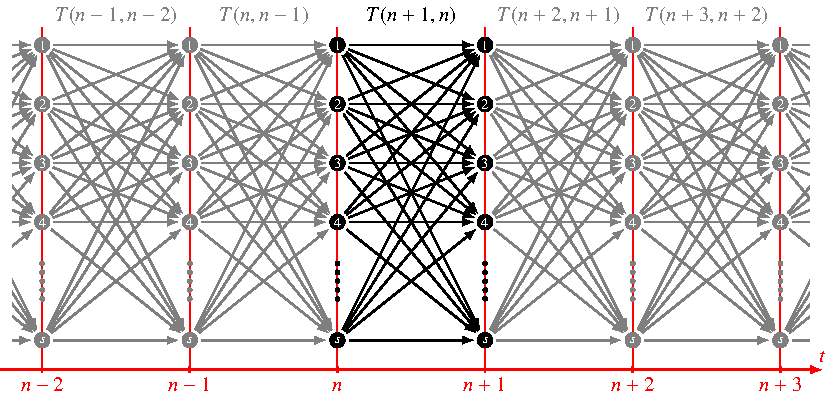
\includegraphics{chapters/80-wahrscheinlichkeit/images/markov.pdf}
\caption{Diskrete Markovkette mit Zuständen $\mathcal{S}=\{1,2,3,\dots,s\}$
und Übergangsmatrizen $T(n+1,n)$.
\label{buch:wahrscheinlichkeit:fig:diskretemarkovkette}}
\end{figure}

Die transienten Übergangswahrscheinlichkeiten zwischen aufeinanderfolgenden
Zeitpunkten stellen jetzt die vollständige Information über die
zeitliche Entwicklung dar
(Abbildung~\ref{buch:wahrscheinlichkeit:fig:diskretemarkovkette}).
Aus der Matrix
\[
T(n+1,n)
=
\begin{pmatrix}
p_{11}(n+1,n) & \dots  & p_{1s}(n+1,n)\\
\vdots        & \ddots & \vdots       \\
p_{s1}(n+1,n) & \dots  & p_{ss}(n+1,n)
\end{pmatrix},
\]
auch die $1$-Schritt-Übergangswahrscheinlichkeit genannt, kann man jetzt
auch die Matrix der Überganswahrscheinlichkeiten für mehrere Schritte
\index{Ubergangswahrscheinlichkeit@Übergangswahrscheinlichkeit}%
\[
T(n+m,n)
=
T(n+m,n+m-1)
T(n+m-1,n+m-2)
\dots
T(n+1,n)
\]
mit der Chapman-Komogorov-Formel bestimmen.
Die Markov-Eigenschaft stellt also sicher, dass man nur die 
$1$-Schritt-Übergangswahrscheinlichkeiten kennen muss.

Eine Matrix $T$ kann als Matrix der Übergangswahrscheinlichkeiten
verwendet werden, wenn sie zwei Bedingungen erfüllt:
\begin{enumerate}
\item Die Einträge von $T$ müssen als Wahrscheinlichkeiten interpretiert
werden können, sie müssen also alle zwischen $0$ und $1$ sein:
$0\le t_{i\!j}\le 1$ für $i,j\in\mathcal{S}$
\item Die Matrix muss alle möglichen Fälle erfassen.
Dazu ist notwendig, dass sich die Wahrscheinlichkeiten aller Übergänge
aus einem Zustand $j$ zu $1$ summieren, also
\[
\sum_{i\in\mathcal{S}} p_{i\!j} = 1.
\]
Die Summe der Elemente einer Spalte 
\end{enumerate}

\begin{beispiel}
Die Permutationsmatrix einer Permutation $\sigma\in S_n$ 
(Abschnitt~\ref{buch:section:permutationsmatrizen})
\index{Permutationsmatrix}%
ist eine Matrix mit Einträgen $0$ und $1$, so dass die erste Bedingung
erfüllt ist.
In jeder Zeile oder Spalte kommt genau eine $1$ vor, so dass auch die
zweite Bedingung erfüllt ist.
Eine Permutationsmatrix beschreibt einen stochastischen Prozess, dessen
Übergänge deterministisch sind.
\end{beispiel}

\subsubsection{Zustandswahrscheinlichkeiten}
Die Wahrscheinlichkeiten, mit der sich der Prozess zum Zeitpunkt $n$
in den Zuständen $i\in\mathcal{S}$ befindet, werden
\[
p_i(n)
=
P(X_i=n)
\]
geschrieben, die auch in einem Vektor $p(n)$ mit den Komponenten
$p_i(n)$ zusammengefasst werden können.
Die Matrix der Übergangswahrscheinlichkeiten erlaubt, die Verteilung
$p(n+1)$ aus der Verteilung $p(n)$ zu berechnen.
Nach dem Satz von der totalen Wahrscheinlichkeit ist nämlich
\[
P(X_{n+1}=x)
=
\sum_{y\in\mathcal{S}} 
P(X_{n+1}=x\mid X_n=y) P(X_n=y)
\qquad\text{oder}\qquad
p(n+1) = T(n+1,n) p(n)
\]
in Matrixform.
Die Zeitentwicklung kann also durch Multiplikation mit der Übergangsmatrix
berechnet werden.

\subsubsection{Zeitunabhängige Übergangswahrscheinlichkeiten}
\index{zeitunabhängige Übergangswahrscheinlichkeiten}
Besonderes einfach wird die Situation, wenn die Übergangsmatrix $T(n+1,n)$
nicht von der Zeit abhängt.
In diesem Fall ist $T(n+1,n) = T$ für alle $n$.
Eine solche Markov-Kette heisst {\em homogen}.
\index{homogene Markov-Kette}%
Die Mehrschritt-Übergangswahrscheinlichkeiten sind dann gegeben
durch die Matrix-Potenzen $T(n+m,n)=T^m$.
Im Folgenden gehen wir immer von einer homogenen Markov-Kette aus.

\subsubsection{Stationäre Verteilung}
Im Beispiel der Google-Matrix erwarten wir intuitiv, dass sich mit
der Zeit eine Verteilung einstellt,  die sich über die Zeit nicht
mehr ändert.
Ein solche Verteilung heisst stationär.

\begin{definition}
Eine Verteilungsvektor $p$ heisst {\em stationär} für die
homogene Markov-Kette mit Übergangsmatrix $T$, wenn $Tp=p$.
\index{stationäre Verteilung}%
\end{definition}

Eine stationäre Verteilung ist offenbar ein Eigenvektor der Matrix
$T$ zum Eigenwert $1$.
Gefunden werden kann er als Lösung des Gleichungssystems $Tp=p$.
Dazu muss aber die Matrix $T-I$ singulär sein, wie man wie folgt
einsehen kann.
Die Summe einer Spalte von $T$ ist aber immer $1$, da sich die
Wahrscheinlichkeiten zu $1$ summieren müssen.
Da die Einheitsmatrix $I$ in jeder Spalte
genau eine $1$ enthält, ist die Summe der Einträge einer Spalte von
$I$ ebenfalls $1$.
Die Summe einer Spalte von $T-I$ ist folglich $0$.
Die Summe aller Zeilen von $T-I$ ist also $0$, die Matrix $T-I$ 
ist singulär.

Dass $T-I$ singulär ist, garantiert aber noch nicht,
dass alle Einträge in einem Eigenvektor zum Eigenwert $1$
auch tatsächlich nichtnegativ gewählt werden können.
Die Perron-Frobenius-Theorie von
\index{Perron-Frobenius-Theorie}%
Abschnitt~\ref{buch:section:positive-vektoren-und-matrizen}
beweist, dass genau dies immer möglich ist.

Es ist nicht garantiert, dass eine stationäre Verteilung
auch eindeutig bestimmt ist.
Dieser Fall tritt immer ein, wenn die geometrische Vielfachheit
des Eigenwerts $1$ grösser ist als $1$.
In Abschnitt~\ref{buch:subsection:elementare-eigenschaften}
werden Bedingungen an eine Matrix $T$ untersucht, die garantieren,
dass der Eigenraum zum Eigenvektor $1$ eindimensional ist.

\begin{beispiel}
Als Beispiel dafür, dass der Eigenraum $\mathcal{E}_1(T)$
mehrdimensional sein kann, betrachten wir eine Permutation $\sigma\in S_n$
\index{Permutation}%
und die zugehörige Permutationsmatrix $P_\sigma$,
\index{Permutationsmatrix}%
wie sie in Abschnitt~\label{buch:section:permutationsmatrizen}
beschrieben worden ist.
Wir verwenden die 
Zyklenzerlegung (Abschnitt~\ref{buch:subsection:zyklenzerlegung})
\(
[n] = \{ Z_1, Z_2,\dots \}
\)
der Permutation $\sigma$, ist ist also $\sigma(Z_i) = Z_i$ für alle
Zyklen.

Jede Verteilung $p$, die auf jedem Zyklus konstant ist, ist eine
stationäre Verteilung.
Ist nämlich $i\in Z_k$, dann ist natürlich auch $\sigma(i)\in Z_k$,
und damit ist $p_{\sigma(i)}=p_i$.

Für jede Wahl von nichtnegativen Zahlen $z_i$ für $i=1,\dots,k$
mit der Eigenschaft $z_1+\dots+z_k=1$ kann man eine stationäre
Verteilung $p(z)$ konstruieren, indem man
\[
p_i(z)
=
\frac{z_i}{|Z_r|}
\qquad\text{wenn}\quad i\in Z_r
\]
setzt.
Die Konstruktion stellt sicher, dass sich die Komponenten zu $1$
summieren.
Wir können aus dem Beispiel auch ableiten, dass die geometrische
Vielfachheit des Eigenwerts $1$ einer Permutationsmatrix $P_\sigma$ 
mindestens so gross ist wie die
Anzahl der Zyklen der Permutation $\sigma$.
\end{beispiel}

\subsubsection{Irreduzible Markov-Ketten}
Die Zyklen-Zerlegung einer Permutation bildet voneinander isolierte
Mengen von Zuständen, es gibt keine Möglichkeit eines Übergangs zu
einem anderen Zyklus.
Die Zyklen können daher unabhängig voneinander studiert werden.
Diese Idee kann auf allgemeine Markov-Ketten verallgemeinert werden.

\begin{definition}
Zwei Zustände $i,j\in\mathcal{S}$ {\em kommunizieren}, wenn die
\index{kommunizieren}%
Übergangswahrscheinlichkeiten $T_{i\!j}(n) \ne 0$ und $T_{i\!j}(n)\ne 0$ sind
für $n$ gross genug.
\end{definition}

Die Zustände, die zu verschiedenen Zyklen einer Permutation gehören,
kommunizieren nicht.
Gerade deshalb waren auch die verschiedenen stationären Verteilungen
möglich.
Eine eindeutige stationäre Verteilung können wir also nur erwarten,
wenn alle Zustände miteinander kommunizieren.

\begin{definition}
Eine homogene Markov-Kette heisst {\em irreduzibel},
wenn alle Zustände miteinander kommunizieren.
\index{irreduzible Markov-Kette}
\end{definition}

\begin{figure}
\centering
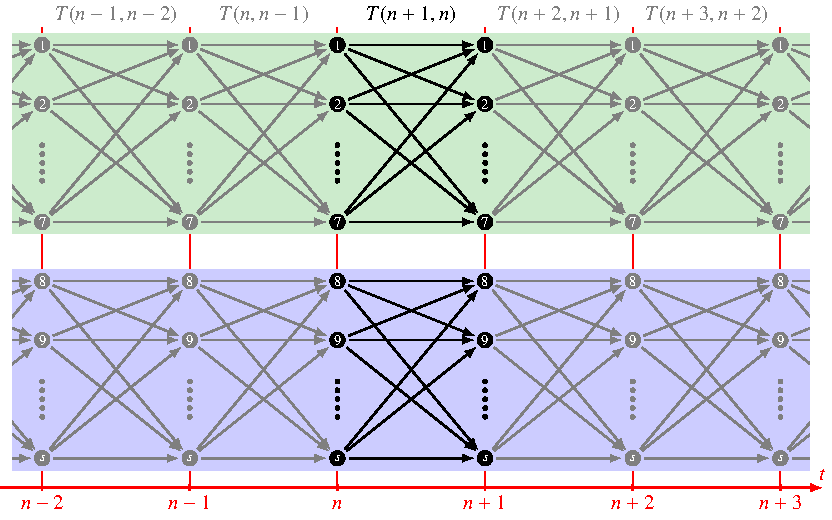
\includegraphics{chapters/80-wahrscheinlichkeit/images/markov2.pdf}
\caption{Diese Markov-Kette zerfällt in zwei verschiedene irreduzible
Markov-Ketten (blau und grün hinterlegt),
deren Zustandsmengen nicht miteinander kommunizieren.
Solche Markov-Ketten können unabhängig voneinander studiert werden.
\label{buch:wahrscheinlichkeit:fig:markovzerfall}}
\end{figure}

Die Bedingung der Irreduzibilität ist gleichbedeutend damit,
dass für genügend grosses $n$ alle Matrixelemente von $T^n$ positiv sind.
Solche Matrizen nennt man {\em positiv}, 
\index{positive Matrix}%
in Abschnitt~\ref{buch:section:positive-vektoren-und-matrizen}
wird gezeigt, dass positive Matrizen immer eine eindeutige
stationäre Verteilung haben.
In Abbildung~\ref{buch:wahrscheinlichkeit:fig:markovzerfall}
ist eine reduzible Markov-Kette dargestellt, die Zustandsmenge
\index{reduzible Markov-Kette}%
zerfällt in zwei Teilmengen von Zuständen, die nicht miteinander
kommunizieren.
Ein irreduzible Markov-Kette liegt vor, wenn sich ähnlich wie
in Abbildung~\ref{buch:wahrscheinlichkeit:fig:diskretemarkovkette}
jeder Zustand von jedem anderen aus erreichen lässt.

Wenn sich der Vektorraum $\mathbb{R}^n$ in zwei unter $T$ invariante
Unterräume zerlegen lässt, dann hat nach Wahl von Basen in den Unterräumen
die Matrix $T$ die Form
\[
\left(
\begin{array}{c|c}
T_1&0\\
\hline
0&T_2
\end{array}
\right).
\]
Insbesondere kann man stationäre Verteilungen von $T_1$ und $T_2$ 
unabhängig voneinander suchen.
Ist $p_i$ eine stationäre Verteilung von $T_i$, dann ist
\[
T
\left(
\begin{array}{c}
g_1p_1\\
\hline g_2p_2
\end{array}
\right)
=
\left(
\begin{array}{c}
g_1T_1p_1\\
\hline
g_2T_2p_2
\end{array}
\right)
=
\left(
\begin{array}{c}
g_1p_1\\
\hline
g_2p_2
\end{array}
\right),\qquad
\text{ für $g_i\in\mathbb{R}$.}
\]
Durch Wahl der Gewichte $g_i\ge 0$ mit $g_1+g_2=1$ lassen sich so
die stationären Verteilungen für $T$ aus den stationären Verteilungen
der $T_i$ ermitteln.
Das Problem, die stationären Verteilungen von $T$ zu finden, ist
auf die Untermatrizen $T_i$ reduziert worden.

\subsubsection{Die konvexe Menge der stationären Verteilungen}
\begin{figure}
\centering
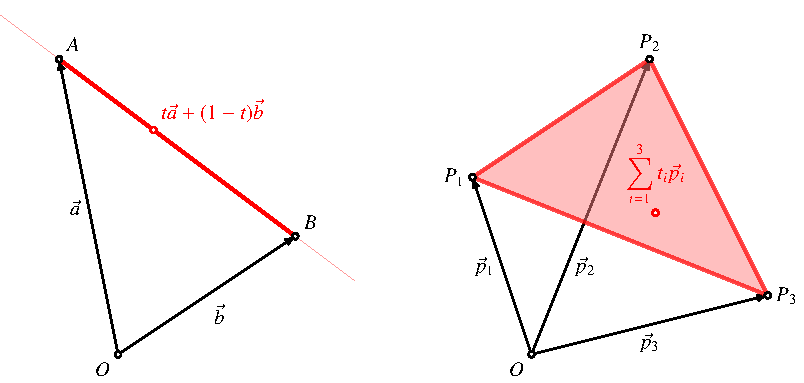
\includegraphics{chapters/80-wahrscheinlichkeit/images/konvex.pdf}
\caption{Die Konvexe Kombination von Vektoren $\vec{p}_1,\dots,\vec{p}_n$ ist
eine Summe der Form $\sum_{i=1}^n t_i\vec{p}_i$ wobei die $t_i\ge 0$
sind mit $\sum_{i=1}^nt_i=1$.
Für zwei Punkte bilden die konvexen Kombinationen die Verbindungsstrecke
zwischen den Punkten, für drei Punkte in drei Dimensionen spannen die
konvexen Kombinationen ein Dreieck auf.
\label{buch:wahrscheinlichkeit:fig:konvex}}
\end{figure}
Die stationären Verteilungen
\[
\operatorname{Stat}(T)
=
\{
p\in\mathbb R_+^n \mid \text{$Tp=p $ und $\|p\|_1=1$}
\}
\]
bilden was man eine konvexe Menge nennt.
Sind nämlich $p$ und $q$ stationäre Verteilungen, dann gilt zunächst
$Tp=p$ und $Tq=q$.
Wegen der Linearität gilt aber auch $T(tp+(1-t)q)=tTp + (1-t)Tq
=tp+(1-t)q$.
Jede Verteilung auf der ``Verbindungsstrecke'' zwischen den beiden
Verteilungen ist auch wieder stationär.

\begin{definition}
Eine {\em konvexe Kombination} von Vektoren $v_1,\dots,v_k\in\mathbb{R}^n$
ist ein Vektor der Form
\[
v=t_1v_1+\dots + t_kv_k
\qquad\text{mit}\quad
t_i\ge 0\;\text{und}\;
t_1+\dots+t_n = 1.
\]
\index{konvexe Kombination}%
Eine Teilmenge $M\subset \mathbb{R}^n$ heisst konvex, wenn zu
zwei Vektoren $x,y\in M$ auch jede konvexe Kombination von $x$ und $y$
wieder in $M$ ist.
\index{konvex}%
\end{definition}

Die konvexen Kombinationen der Vektoren sind Linearkombination
mit nichtnegativen Koeffizienten. Sie bilden im Allgemeinen
einen $(k-1)$-Simplex in $\mathbb{R}^n$ (siehe auch
Abbildung~\ref{buch:wahrscheinlichkeit:fig:konvex}).
Für zwei Punkte $x$ und $y$ bilden die konvexen Kombination
$tx+(1-t)y$ für $t\in[0,1]$ die Verbindungsstrecke der beiden
Vektoren.
Eine Menge ist also konvex, wenn sie mit zwei Punkten immer auch
ihre Verbindungsstrecke enthält.
% XXX Bild für konvexe Mengen

\subsubsection{Grenzverteilung}
Im Beispiel der Google-Matrix wurde ein iterativer Algorithmus
zur Berechnung des Pagerank verwendet.
Es stellt sich daher die Frage, ob diese Methode für andere homogene
Markov-Ketten auch funktioniert.
Man beginnt also mit einer beliebigen Verteilung $p(0)$ und wendet
die Übergangsmatrix $T$ wiederholt an.
Es entsteht somit eine Folge $p(n) = T^np(0)$.

\begin{definition}
Falls die Folge $p(n) = T^np(0)$ konvergiert, heisst der Grenzwert
\[
p(\infty) = \lim_{n\to\infty} p(n)
\]
eine {\em Grenzverteilung} von $T$.
\index{Grenzverteilung}%
\end{definition}

Falls eine Grenzverteilung existiert, dann ist sie eine stationäre
Verteilung.
Für eine stationäre Verteilung $p(0)$ ist die Folge $p(n)$ eine
konstante Folge, sie konvergiert also gegen $p(0)$.
Stationäre Verteilungen sind also automatisch Grenzverteilungen.
Falls der Raum der stationären Verteilungen mehrdimensional ist,
braucht die Grenzverteilung nicht eindeutig bestimmt zu sein, selbst
wenn sie existiert.
Aber nicht einmal die Existenz einer Grenzverteilung ist garantiert,
wie das folgende Beispiel zeigt.

\begin{beispiel}
Sei $T$ die Permutationsmatrix der zyklischen Verteilung von drei
Elementen in $S_3$, also die Matrix
\[
T=\begin{pmatrix}
0&0&1\\
1&0&0\\
0&1&0
\end{pmatrix}.
\]
Die konstante Verteilung $\frac13U$ ist offensichtlich eine
stationäre Verteilung.
In Abschnitt~\ref{buch:section:positive-vektoren-und-matrizen}
wird gezeigt, dass es die einzige ist.
Sei jetzt $p(0)$ ein beliebiger Vektor in $\mathbb{R}^3$ mit
nichtnegativen Einträgen, die sich zu $1$ summieren.
Dann bilden die Vektoren $p(n)=T^np(0)$ einen Dreierzyklus
\begin{align*}
p(0)&=p(3)=p(6)=\dots =\begin{pmatrix}p_1(0)\\p_2(0)\\p_3(0)\end{pmatrix},
\\
p(1)&=p(4)=p(7)=\dots =\begin{pmatrix}p_2(0)\\p_3(0)\\p_1(0)\end{pmatrix},
\\
p(2)&=p(5)=p(8)=\dots =\begin{pmatrix}p_3(0)\\p_1(0)\\p_2(0)\end{pmatrix}.
\end{align*}
Die Folge $p(n)$ kann also nur dann konvergieren, wenn die drei
Komponenten gleich sind.
Insbesondere gibt es keine Grenzverteilung, wenn sie nicht alle
gleich sind.
\end{beispiel}

\subsubsection{Erwartungswert und Varianz}
Wenn sich im Laufe der Zeit eine Grenzverteilung einstellen soll, dann
muss es auch möglich sein, Erwartungswert und Varianz dieser Verteilung
zu berechnen.
Dazu muss jedem Zustand ein Zahlenwert zugeordnet werden.
Sei also
\(
g: \mathcal{S}\to \mathbb{R}
\)
eine Funktion, die einem Zustand eine reelle Zahl zuordnet.
Aus der Zufallsvariable $X_n$ des Zustands zur Zeit $n$ wird daraus
die reellwertige Zufallsvariable $Y_n=g(X_n)$ des Wertes zur Zeit $n$.
Die Abbildung $g$ kann auch als Vektor mit der Komponenten $g_i$ 
für $i\in\mathcal{S}$ betrachtet werden, wir verwenden für diesen
Vektor wieder die Schreibweise $g$.

Für die Verteilung $p(n)$ kann man jetzt auch Erwartungswert und
Varianz berechnen.
Der Erwartungswert ist
\[
E(Y)
=
\sum_{i\in\mathcal{S}} g_i p_i(n)
=
g^t p(n).
\]
Für die Varianz muss $g_i$ durch $g_i^2$ ersetzt werden.
Dies kann am einfachsten mit dem Hadamard-Produkt geschrieben werden:
\begin{align*}
E(Y^2)
&=
\sum_{i\in\mathcal{S}} g_i p_i(n)
=
(g\odot g)^t p(n)
\\
E(Y^k)
&=
(g^{\odot k})^t p(n),
\end{align*}
wobei wir die Hadamard-Potenz $A^{\odot k}$ einer Matrix $A$ rekursiv
durch
\[
A^{\odot 0}=U
\qquad\text{und}\qquad
A^{\odot k} = A\odot A^{\odot (k-1)}
\]
definieren.

\subsubsection{Erwartungswert von Werten auf Übergängen}
In Abschnitt~\ref{buch:section:paradoxon-von-parrondo} wird ein Spiel
vorgestellt, in dem der Gewinn davon abhängt, welcher Übergang stattfindet,
nicht welcher Zustand erreicht wird.
Es git daher eine Matrix $G$ von Gewinnen, der Eintrag $g_{i\!j}$ ist
der Gewinn, der bei einem Übergang von Zustand $j$ in den Zustand $i$
ausgezahlt wird.
Mit dieser Matrix lassen sich jetzt viele verschiedene Fragen beantworten:

\begin{frage}
\label{buch:wahrscheinlichkeit:frage1}
Mit welchem Gewinn kann man in Runde $n$ des Spiels rechnen,
wenn die Verteilung zur Zeit $n-1$ durch $p(n-1)$ gegeben ist?
\end{frage}

Der Erwartungswert ist
\begin{align*}
E(Y)
&=
\sum_{i,j\in\mathcal{S}}
g_{ji} t_{ji} p_i(n-1)
\intertext{oder in Matrixform}
&=
U^t
(G\odot T)
p(n-1).
\end{align*}

\begin{frage}
Mit welchen Gewinnen kann man rechnen, wenn der Prozess sich zu Beginn 
einer Spielrunde im Zustand $i$ befindet?
\end{frage}

Dies ist der Spezialfall der Frage~\ref{buch:wahrscheinlichkeit:frage1}
für die Verteilung $p_j(n-1) = \delta_{i\!j}$.
Der Erwartungswert ist die Summe der Spalte $j$ der Matrix $G\odot T$.
Man kann das Produkt $U^t(G\odot T)$ also auch als eine Zeilenvektor
von Gewinnerwartungen unter der Vorbedingung $X_{n-1}=j$ betrachten:
\[
\begin{pmatrix}
E(Y\mid X_{n-1}=1)
&\dots&
E(Y\mid X_{n-1}=n)
\end{pmatrix}
=
U^t (G\odot T).
\]
Indem man $G$ durch $G^{\odot k}$ ersetzt, kann man beliebige höhere
Momente berechnen.

\subsection{Absorbierende Zustände}
In diesem Abschnitt gehen wir immer von einer irreduziblen, homogenen
Markov-Kette aus.
Ihre Übergangsmatrix enthält die Wahrscheinlichkeiten
\[
T_{i\!j}
=
P(X_{k+1}=i\mid X_{k}=j)
\]
für alle Zeiten $k$.

Eine Grenzverteilung beschreibt die relative Häufigkeit, mit der
der Prozess in den verschiedenen Zuständen vorbeikommt.
In einem Spiel, in dem der Spieler ruiniert werden kann, gibt es
aus dem Ruin-Zustand keinen Weg zurück.
Der Spieler bleibt in diesem Zustand.

\begin{definition}
Ein Zustand $i$ einer homogenen Markov-Kette mit Übergangsmatrix $T$
heisst {\em absorbierend}, wenn $T_{ii}=1$ ist.
\index{absorbierender Zustand}%
Eine Markov-Kette mit mindestens einem absorbierenden Zustand heisst
{\em absorbierende Markov-Kette}.
\index{absorbierende Markov-Kette}%
Nicht absorbierende Zustände heissen {\em transient}.
\index{transienter Zustand}%
\end{definition}

\begin{figure}
\centering
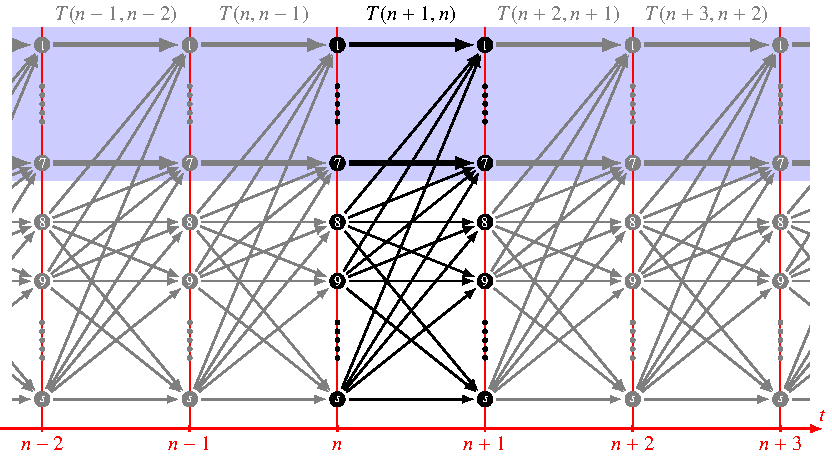
\includegraphics{chapters/80-wahrscheinlichkeit/images/markov3.pdf}
\caption{Markov-Kette mit absorbierenden Zuständen (blau hinterlegt).
Erreicht die Markov-Kette einen absorbierenden Zustand, dann verbleibt
sie für alle zukünftigen Zustände in diesem Zustand.
\label{buch:wahrscheinlichkeit:fig:abs}}
\end{figure}

Eine Markov-Kette kann mehrere absorbierende Zustände haben, wie in
Abbildung~\ref{buch:wahrscheinlichkeit:fig:abs} dargestellt.
Indem man die absorbierenden Zustände zuerst auflistet, gefolgt von
den transienten Zustädnen, bekommt die Übergangsmatrix die Form
\[
T=
\left(
\begin{array}{c|c}
I&R\\
\hline
0&Q
\end{array}
\right).
\]
Die Matrix $R$ beschreibt die Wahrscheinlichkeiten, mit denen man
ausgehend von einem transienten Zustand
in einem bestimmten absorbierenden Zustand landet.
Die Matrix $Q$ beschreibt die Übergänge, bevor dies passiert.
Die Potenzen von $T$ sind
\begin{equation}
T^2
=
\left(
\begin{array}{c|c}
I&R+RQ \\
\hline
0&Q^2
\end{array}
\right),
\quad
T^3
=
\left(
\begin{array}{c|c}
I&R+RQ+RQ^2 \\
\hline
0&Q^3
\end{array}
\right),
\;
\dots,
\;
T^k
=
\left(
\begin{array}{c|c}
I&\displaystyle R\sum_{l=0}^{k-1} Q^l \\
\hline
0&Q^k
\end{array}
\right).
\label{buch:markov:eqn:Tpowers}
\end{equation}
Die Potenzen enthalten die Wahrscheinlichkeiten
\[
(T^k)_{i\!j}
=
P(X_k=i\mid X_0=j),
\]
dass der Prozess ausgehend vom Zustand $j$ im Schritt $k$ im
Zustand $i$ ankommt.

Wegen der angenommenen Irreduzibilität wird man
früher oder später in einem absorbierenden Zustand landen,
daher muss $\lim_{k\to\infty} Q^k=0$ sein.
Die Summe in der rechten oberen Teilmatrix kann man als geometrische
Reihe summieren, man erhält die Matrix
\[
\sum_{l=0}^{k-1} Q^l = (I-Q)^{-1}(I-Q^k),
\]
die für $k\to\infty$ gegen
\[
F
=
\lim_{k\to\infty} \sum_{l=0}^{k-1} Q^l
=
(I-Q)^{-1}
\]
konvergiert.
Die Matrix $F$ heisst die {\em Fundamentalmatrix} der absorbierenden
Markov-Kette.
\index{Fundamental-Matrix}%
Sie gestattet, viele interessante Grössen des Markov-Prozesses zu
berechnen.

\subsubsection{Erwartete Anzahl Besuche eines Zustandes}
Wie häufig wird ein Zustand $i$ ausgehend von einem Zustand $j$
besucht?
\index{Anzahl Besuche}%
Dazu definieren wir die ``Besuchs''-Zufallsvariable
\[
B_{k}=\begin{cases}
1&\qquad\text{$X_k=i$}\\
0&\qquad\text{sonst,}
\end{cases}
\]
die genau dann $1$ ist, wenn der Prozess ausgehend vom Zustand $j$
beim $k$-ten Schritt den Zustand $i$ besucht.
Die Zufallsvariable der Anzahl $B$ der Besuche des Zustands $i$ ist die
Summe der $B_k$.
Ein weiterer Nutzen dieser Definition ist, dass sich die Wahrscheinlichkeit
jetzt als Erwartungswert ausdrücken lässt, es ist
$P(X_k=i \mid X_0=j) = E(B_k)$.

Damit lässt sich jetzt die Fundamentalmatrix auf andere Art interpretieren.
Der Eintrag $F_{i\!j}$ ist
\begin{align*}
F_{i\!j}
&=
\biggl(\sum_{k=0}^\infty Q^k\biggr)_{i\!j}
\\
&=
P(X_0=i\mid X_0=j)
+
P(X_1=i\mid X_0=j)
+
P(X_2=i\mid X_0=j)
+\dots
\\
&=E(B_0) + E(B_1) + E(B_2) + \dots
\\
&=E(B_0+B_1+B_2+\dots)
=E(B).
\end{align*}
Die Summe der $B_k$ ist die erwartete Anzahl der Besuch im Zustand $i$.

\begin{satz}
\label{buch:markov:satz:anzahlbesuche}
Die erwartete Anzahl Besuche des Zustands $i$ eines homogenen,
absorbierenden Markovprozesses ausgehend vom Zustand $j$ ist das
Element $F_{i\!j}$ der Fundamentalmatrix $F=(I-Q)^{-1}$.
\end{satz}

\subsubsection{Absorptionszeit}
\index{Absorptionszeit}%
\begin{frage}
Wie lange dauert es im Mittel, bis der Prozess ausgehend vom Zustand $j$
in einem Absorbptionszustand $i$ stecken bleibt?
\end{frage}
Die Absorptionszeit ist gleich gross wie die Zeit,
während der der Prozess nicht absorbierende
Zustände besucht.
Die Zeit $t_j$, bis der Prozess in einen absorbierenden Zustand wechselt, ist also
die erwartete Anzahl Besuche nicht absorbierender Zustände.
Es folgt:
\[
t_j
=
\sum_{\text{$i$ nicht absorbierend}} E(\text{Anzahl Besuche von $i$}\mid X_0=j)
=
\sum_{i} F_{i\!j}.
\]
$t_j$ ist also die Summe der Elemente der Spalte $j$ der Fundamentalmatrix $F$.
Man kann diese Summe auch vektoriell schreiben mit einem Zeilenvektor $U^t$
aus lauter Nullen.
Der Zeilenvektor $t$ mit Einträgen $t_j$ ist dann
\(
t = U^tF.
\)
\begin{satz}
\label{buch:markov:satz:absorptionszeit}
Die Absorptionszeit $t_j$ einer absorbierenden, homogenen Markov-Kette
ausgehend vom Zustand $j$ ist
das $j$-te Element des Zeilenvektors $U^tF$ oder die Summe der
Einträge in Spalte $j$ der Fundamentalmatrix $F$.
\end{satz}

\subsubsection{Absorptionswahrscheinlichkeit}
\index{Absorptionswahrscheinlichkeit}%
\begin{frage}
Wie gross ist die Wahrscheinlichkeit, dass der Prozess ausgehend von
Zustand $j$ irgendwann im Zustand $i$ absorbiert wird?
\end{frage}
Die Potenzen $T^k$ der Übergangsmatrix enthalten in Zeile $j$
und Spalte $i$ die Wahrscheinlichkeit, dass dies nach spätestens $k$ Schritten
geschehen ist.
Wir müssen daher den Grenzwert
\(
\lim_{k\to\infty}T^k
\)
berechnen.
Da $\|Q\|<1$ folgt aus~\eqref{buch:markov:eqn:Tpowers} sofort
\[
T^\infty
=
\lim_{k\to\infty}T^k
=
\left(
\begin{array}{cc}
I&RF\\
0&0
\end{array}
\right).
\]
Die Matrix $RF$ enthält also in Zeile $i$ und Spalte $j$
die Wahrscheinlichkeit, dass der Prozess ausgehend vom Zustand $j$
irgendwann im Zustand $i$ absorbiert wird.

\subsubsection{Absorption über den letzten Zustand $l$}
\begin{frage}
Wie gross ist die Wahrscheinlichkeit, dass die von $j$ ausgehende
Absorption in den Zustand $i$ als letzten Zustand vor der Absorption
den Zustand $l$ hat?
\end{frage}
Wir schreiben $l\overset{\smash{k}}{\twoheadrightarrow} i$ für das Ereignis, dass der Prozess
im $k$-ten Schritt über den letzten
Zustand $l$ in den Absorbtionszustand $i$ übergeht.
Ist uns der Zeitpunkt des Übergangs egal, lassen wir das $k$
weg und schreiben nur $l\twoheadrightarrow i$.

Damit $l\overset{\smash{k}}{\twoheadrightarrow} i$ eintritt, muss der Prozess im $(k-1)$-ten Schritt im
Zustand $l$ ankommen, was er mit Wahrscheinlichkeit
\[
P(X_{k-1}=l\wedge X_0=j) = (Q^{k-1})_{l\!j}
\]
tut, und dann den Übergang von $l$ nach $i$ nehmen, was er mit
Wahrscheinlichkeit $r_{il}$ tut.
Somit ist die gesuchte Wahrscheinlichkeit
\begin{equation}
P(X_K=i\wedge X_{k-1}=l\wedge X_0=j)
=
P(l\overset{k}{\twoheadrightarrow} i\wedge X_0=j)
=
r_{il}(Q^{k-1})_{l\!j}.
\label{buch:markov:eqn:Pilj}
\end{equation}

Die Wahrscheinlichkeit, dass der Prozess zu irgend einer Zeit von $j$
ausgehend über den letzten Zustand $l$ in den Absorptionszustand $i$
übergeht, ist die Summe der Wahrscheinlichkeiten~\eqref{buch:markov:eqn:Pilj}
für alle $k$.
Der Faktor $r_{il}$ ist all diesen Termen gemeinsam, die Summe der
$Q$-Terme kann wieder durch die Fundamentalmatrix als
\[
P(l\twoheadrightarrow i\wedge X_0 = j)
=
\sum_{k=0}^\infty r_{il}(Q^k)_{l\!j}
=
r_{il}\biggl(\sum_{k=0}^\infty (Q^k)\biggr)_{l\!j}
=
r_{il}F_{l\!j}
\]
geschrieben werden.

\subsubsection{Wartezeit für eine beliebige Markov-Kette}
\index{Wartezeit}%
\begin{frage}
Wie gross ist die mittlere Wartezeit, bis eine beliebige Markov-Kette
einen bestimmten Zustand erreicht?
\end{frage}
Auch diese mittlere Wartezeit kann mit der
Theorie zur Berechnung der Absorptionszeit berechnet werden.
Dazu modifiziert man den Prozess dahingehend, dass der Zielzustand
ein absorbierender Zustand wird.
Der Einfachheit halber gehen wir davon aus, dass der Zustand $1$ 
der Zielzustand ist.
Wir ersetzen die Übergangsmatrix $T$ durch die Matrix
\[
\tilde{T}
=
\left(
\begin{array}{c|ccc}
1     &t_{12}&\dots &t_{1n}\\
\hline
0     &t_{22}&\dots &t_{2n}\\
\vdots&\dots &\ddots&\vdots\\
0     &t_{n2}&\dots &t_{nn}
\end{array}\right).
\]
$\tilde{T}$ hat den Zustand $1$ als absorbierenden Zustand.
Die $Q$ und $R$ sind
\[
\tilde{R}
=
\begin{pmatrix}t_{12}&\dots&t_{1n}\end{pmatrix},
\quad
\tilde{Q}
=
\begin{pmatrix}
t_{22}&\dots &t_{2n}\\
\vdots&\ddots&\vdots\\
t_{n2}&\dots &t_{nn}
\end{pmatrix}.
\]
Die Wartezeit bis zum Erreichen des Zustands $i$ ausgehend von einem
Zustand $n$ kann jetzt aus der Absorbtionszeit der Markov-Kette
im Zustand $1$ mit Hilfe der Fundamentalmatrix
\[
\tilde{F} 
=
(I-\tilde{Q})^{-1}
\]
berechnet werden.


